%ju 31-Dez-22 05-Datenbus.tex
Quelle: Fabian Lindenberg, Kfz-Technik einfach erklärt \footnote{\url{https://www.youtube.com/watch?v=0a33FFpn_eM\&list=PLJXzCsL6HEwzoI3j8tGLKUHjLx0gTxus8}}

\textbf{Früher} für jedes Signal eine Leitung $\to$ viele Kabel
notwendig, wenn mehrere Steuergeräte auf Sensordaten zugreifen wollen.

\textbf{Heute} ein Steuergerät liest die Sensordaten aus und schickt
diese auf den Datenbus. \emph{Beispiel} Motordrehzahlsignal wird von
folgenden Steuergeräten benötigt: Motor, Getriebe, Kombiinstrument,
Klimaanlage, ESP.

\textbf{Datenübertragung im Kfz} Ermöglicht den Transport und Austausch
von Informationen in Form von Daten und Signalen.

\textbf{Gateway} ermöglicht und überwacht den Datenaustausch zwischen
Datenbussysteme mit unterschiedlichen Übertragungsgeschwindigkeiten.

\textbf{Vorteile}

\begin{enumerate}
\item
  gemeinsame Nutzung von Sensoren
\item
  verbesserte Diagnosefähigkeit
\item
  weniger elektrische Leitungen
\item
  weniger Fehlerquellen
\end{enumerate}

\section{Datenbusarten}\label{datenbusarten}

\begin{enumerate}
\item
  \textbf{elektrische Einleiter - Datenbussysteme}: LIN (Local
  Interconnect Network, Master-Slave), Multiplex

  \begin{itemize}
  \item
    Übertragungsart: elektrische Leitung
  \end{itemize}
\item
  \textbf{elektrische Zweileiter - Datenbussysteme}: CAN (Controller
  Area Network), Flexray, Ethernet

  \begin{itemize}
  \item
    Übertragungsart: elektrische Leitung
  \end{itemize}
\item
  \textbf{optische Datenbussysteme}: Glasfaser, MOST

  \begin{itemize}
  \item
    Übertragungsart: Lichtwellen
  \end{itemize}
\item
  \textbf{drahtlose Datenbussysteme}: WLAN, Bluetooth

  \begin{itemize}
  \item
    Übertragungsart: Funkwellen (elektromagnetische Wellen, 2,4 GHZ / 5
    GHz)
  \end{itemize}
\end{enumerate}

\newpage

\section{Datenbusstrukturen - Topologie -
Netzwerkstruktur}\label{datenbusstrukturen-topologie-netzwerkstruktur}

\begin{figure}[!ht]% hier: !ht
\centering
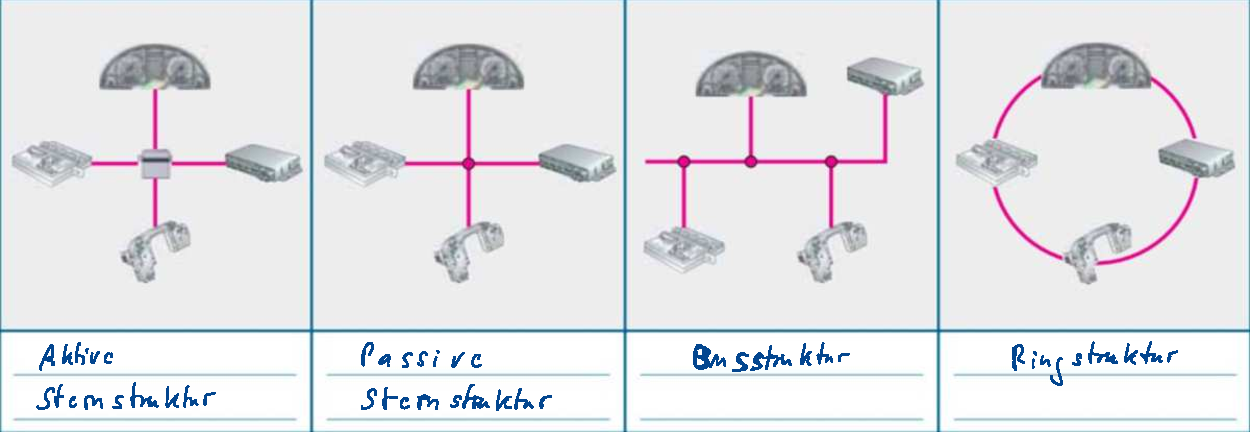
\includegraphics[width=0.5\textwidth]{images/CAN-Bus/CAN-Bus-6.pdf}
\caption{Datenbusstrukturen, Quelle: Europa-Verlag}
%\label{fig:}%% anpassen
\end{figure}

\begin{enumerate}
\item
  \textbf{Sternstruktur:} (Gateway / Router $\leftrightarrow$ PC /
  Handy / Tablet / Drucker usw.)

  \begin{itemize}
  \item
    \textbf{aktiv} (Ein Steuergerät im Zentrum eine sternförmig
    aufgebauten Datennetzes ist über Punkt-zu-Punkt-Verbindungen mit dem
    benachbarten Steuergerät verbunden.), \textbf{passiv}
    (Leitungsknoten in der Mitte)
  \end{itemize}
\item
  \textbf{Daisy-Chain:} Steuergeräte sind wie die Glieder einer
  Kette/Reihe aneinander gereiht. (Gateway $\to$ PC $\to$ PC $\to$
  PC $\to$ TV)
\item
  \textbf{Busstruktur / Linear:} CAN-Bus (Datenbusleitung, Knotenpunkte,
  $SG_1 \Longleftrightarrow SG_2 \Longleftrightarrow SG_3 \Longleftrightarrow SG_n$)
\item
  \textbf{Ringstruktur} (Most) Nachteil: Bei fehlerhaften
  Lichtwellenleiter oder Steuergerät fällt die gesamte Kommunikation
  aus.
\item
  \textbf{Hybrid} (mehrere Busse, Stern-Bus oder Stern-Ring)
\item
  \textbf{Maschen} (hohe Ausfallsicherheit)
\end{enumerate}

\emph{Bemerkung:} Datenbusleitungen sind miteinander verdrillt (twisted
pair), um elektromagnetische Auswirkungen von einem auf den anderen
Draht zu minimieren. Durch die gegensätzliche Spannungsänderung heben
sich die bei jeder Umschaltung entstehenden Magnetfelder beider
Leitungen gegenseitig auf. Die Leitungen sind nach außen
elektromagnetisch neutral. (\textbf{EMV} Elektromagnetischen
Verträglichkeit)

\newpage

\section{Klassifikation von
Bussystemen}\label{klassifikation-von-bussystemen}

\textbf{Nenne Merkmale des CAN-Datenbus}

\begin{enumerate}
\item
  \textbf{Klasse A}

  \begin{itemize}
  \item
    LIN bis 10 kBit/s
  \item
    Vernetzung von Aktoren und Sensoren
  \end{itemize}
\item
  \textbf{Klasse B} (Lowspeed-CAN, CAN-B, Komfortbereich)

  \begin{itemize}
  \item
    bis 125 kBit/s
  \item
    \textbf{Eindrahtfähig} Datenkommunikation ist gegeben, auch wenn
    eine Busleitung ausfällt
  \item
    keine Abschlusswiderstände
  \item
    \textbf{Dominanter Pegel 0} low: 1,4 V und high: 3,6 V (Quelle:
    Bosch S.1693, 30. Auflage)
  \item
    \textbf{Rezessiver Pegel 1} low: 5 V und high: 0 V
  \end{itemize}
\item
  \textbf{Klasse C} (Highspeed-CAN, CAN-C, Antriebs- und
  Fahrwerkbereich)

  \begin{itemize}
  \item
    Datenrate bis 1 MBit/s
  \item
    Nicht Eindrahtfähig
  \item
    Abschlusswiderstand im Steuergerät
  \item
    Leitungen sind verdrillt
  \item
    CAN-High
  \item
    CAN-Low
  \item
    keine Potenzialverteiler
  \item
    oder Potenzialverteiler mit Abschlusswiderständen
  \item
    \textbf{Dominanter Pegel 0} low: 1,5 V und high: 3,5 V (Quelle:
    Bosch S.1693, 30. Auflage)
  \item
    \textbf{Rezessiver Pegel 1} low: 2,5 V und high: 2,5 V
  \end{itemize}
\item
  \textbf{CAN FD} (Flexible Data)

  \begin{itemize}
  \item
    bis ca. 8 MBit/s
  \item
    Erst wenn die Daten kommen, wird die Geschwindigkeit hoch
    geschaltet.
  \end{itemize}
\item
  \textbf{Klasse C+}

  \begin{itemize}
  \item
    FlexRay bis 10 MBit/s
  \item
    Antriebs- und Fahrwerkbereich
  \end{itemize}
\item
  \textbf{Klasse D}

  \begin{itemize}
  \item
    MOST, Ethernet ab 10 MBit/s
  \item
    Telematik-, Multimediabereich
  \end{itemize}
\end{enumerate}

\textbf{Multi-Master} Alle Steuergeräte sind gleichberechtigt. Regelung
erfolgt nach Priorität.

\textbf{Autonomes Fahren} Drive-by-Wire (alle sicherheitsrelevanten
Bauteile sind zweifach ausgelegt und zwei Bussysteme)

\newpage

\section{Aufbau CAN-Bus}\label{aufbau-can-bus}

Steuergerät sendet Nachricht auf den Datenbus.

\begin{figure}[!ht]% hier: !ht
\centering
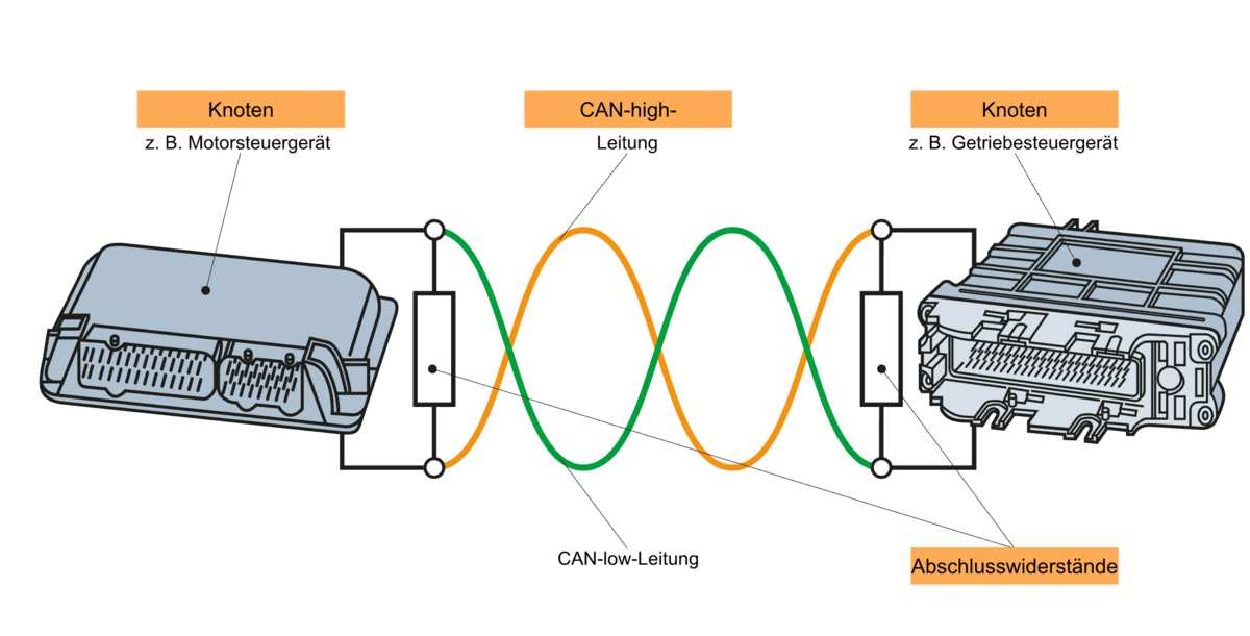
\includegraphics[width=0.6\textwidth]{images/CAN-Bus/CAN-Bus-2.pdf}
\caption{Aufbau CAN-Datenbus, Quelle: Europa-Verlag}
%\label{fig:}%% anpassen
\end{figure}

\begin{figure}[!ht]% hier: !ht
\centering
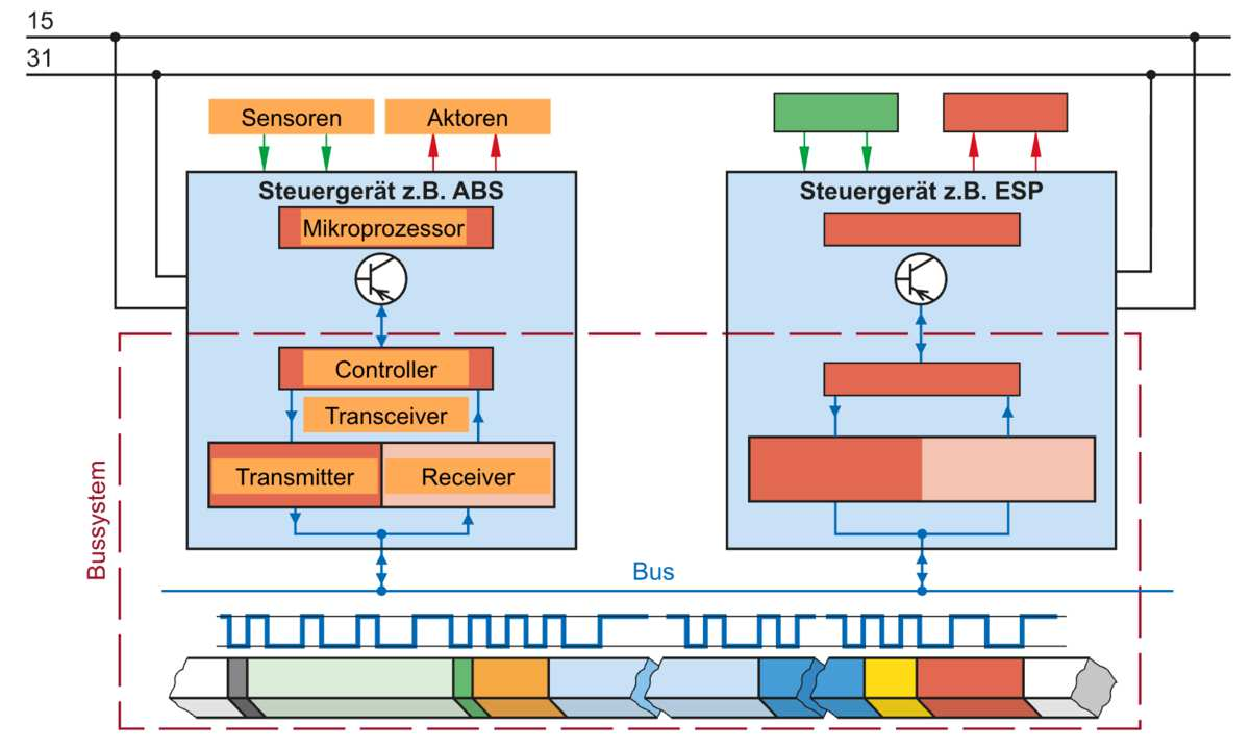
\includegraphics[width=0.6\textwidth]{images/CAN-Bus/CAN-Bus-3.pdf}
\caption{Aufbau-elektrisches-CAN-Datenbussystem, Quelle: Europa-Verlag}
%\label{fig:}%% anpassen
\end{figure}

\textbf{Steuergerät} (Knoten, Busteilnehmer)

\begin{enumerate}
\item
  \textbf{Microprozessor} verarbeitet die eingehenden Informationen,
  berechnet die Funktionen und steuert die Aktoren.
\item
  \textbf{Controller} filtert die für das Steuergerät notwendigen Daten
  und übermittelt sie dem Mikroprozessor.
\item
  \textbf{Transceiver} empfängt und sendet die Daten auf der Busleitung.
  Transmitter (Sender), Receiver (Empfänger)
\end{enumerate}

\newpage

\textbf{Spannungspegel der CAN-Datenübertragung}

Beim CAN-Bussystem werden die Informationen durch Spannungsänderungen in
der Datenleitung übertragen. Dadurch empfangen alle Steuergeräte
gleichzeitig die Informationen. Die Bits werden nacheinander übertragen
(seriell).

\textbf{Zwei Leitungen}

\begin{enumerate}
\item
  \textbf{High-Leitung} Beim Wechsel von rezessiven (Bit = 1) zum
  dominanten (Bit = 0) Pegel steigt die Spannung.
\item
  \textbf{Low-Leitung} Beim Wechsel vom rezessiven (Bit = 1) zum
  dominanten (Bit = 0) Pegel sinkt die Spannung.
\end{enumerate}

\begin{figure}[!ht]% hier: !ht
\centering
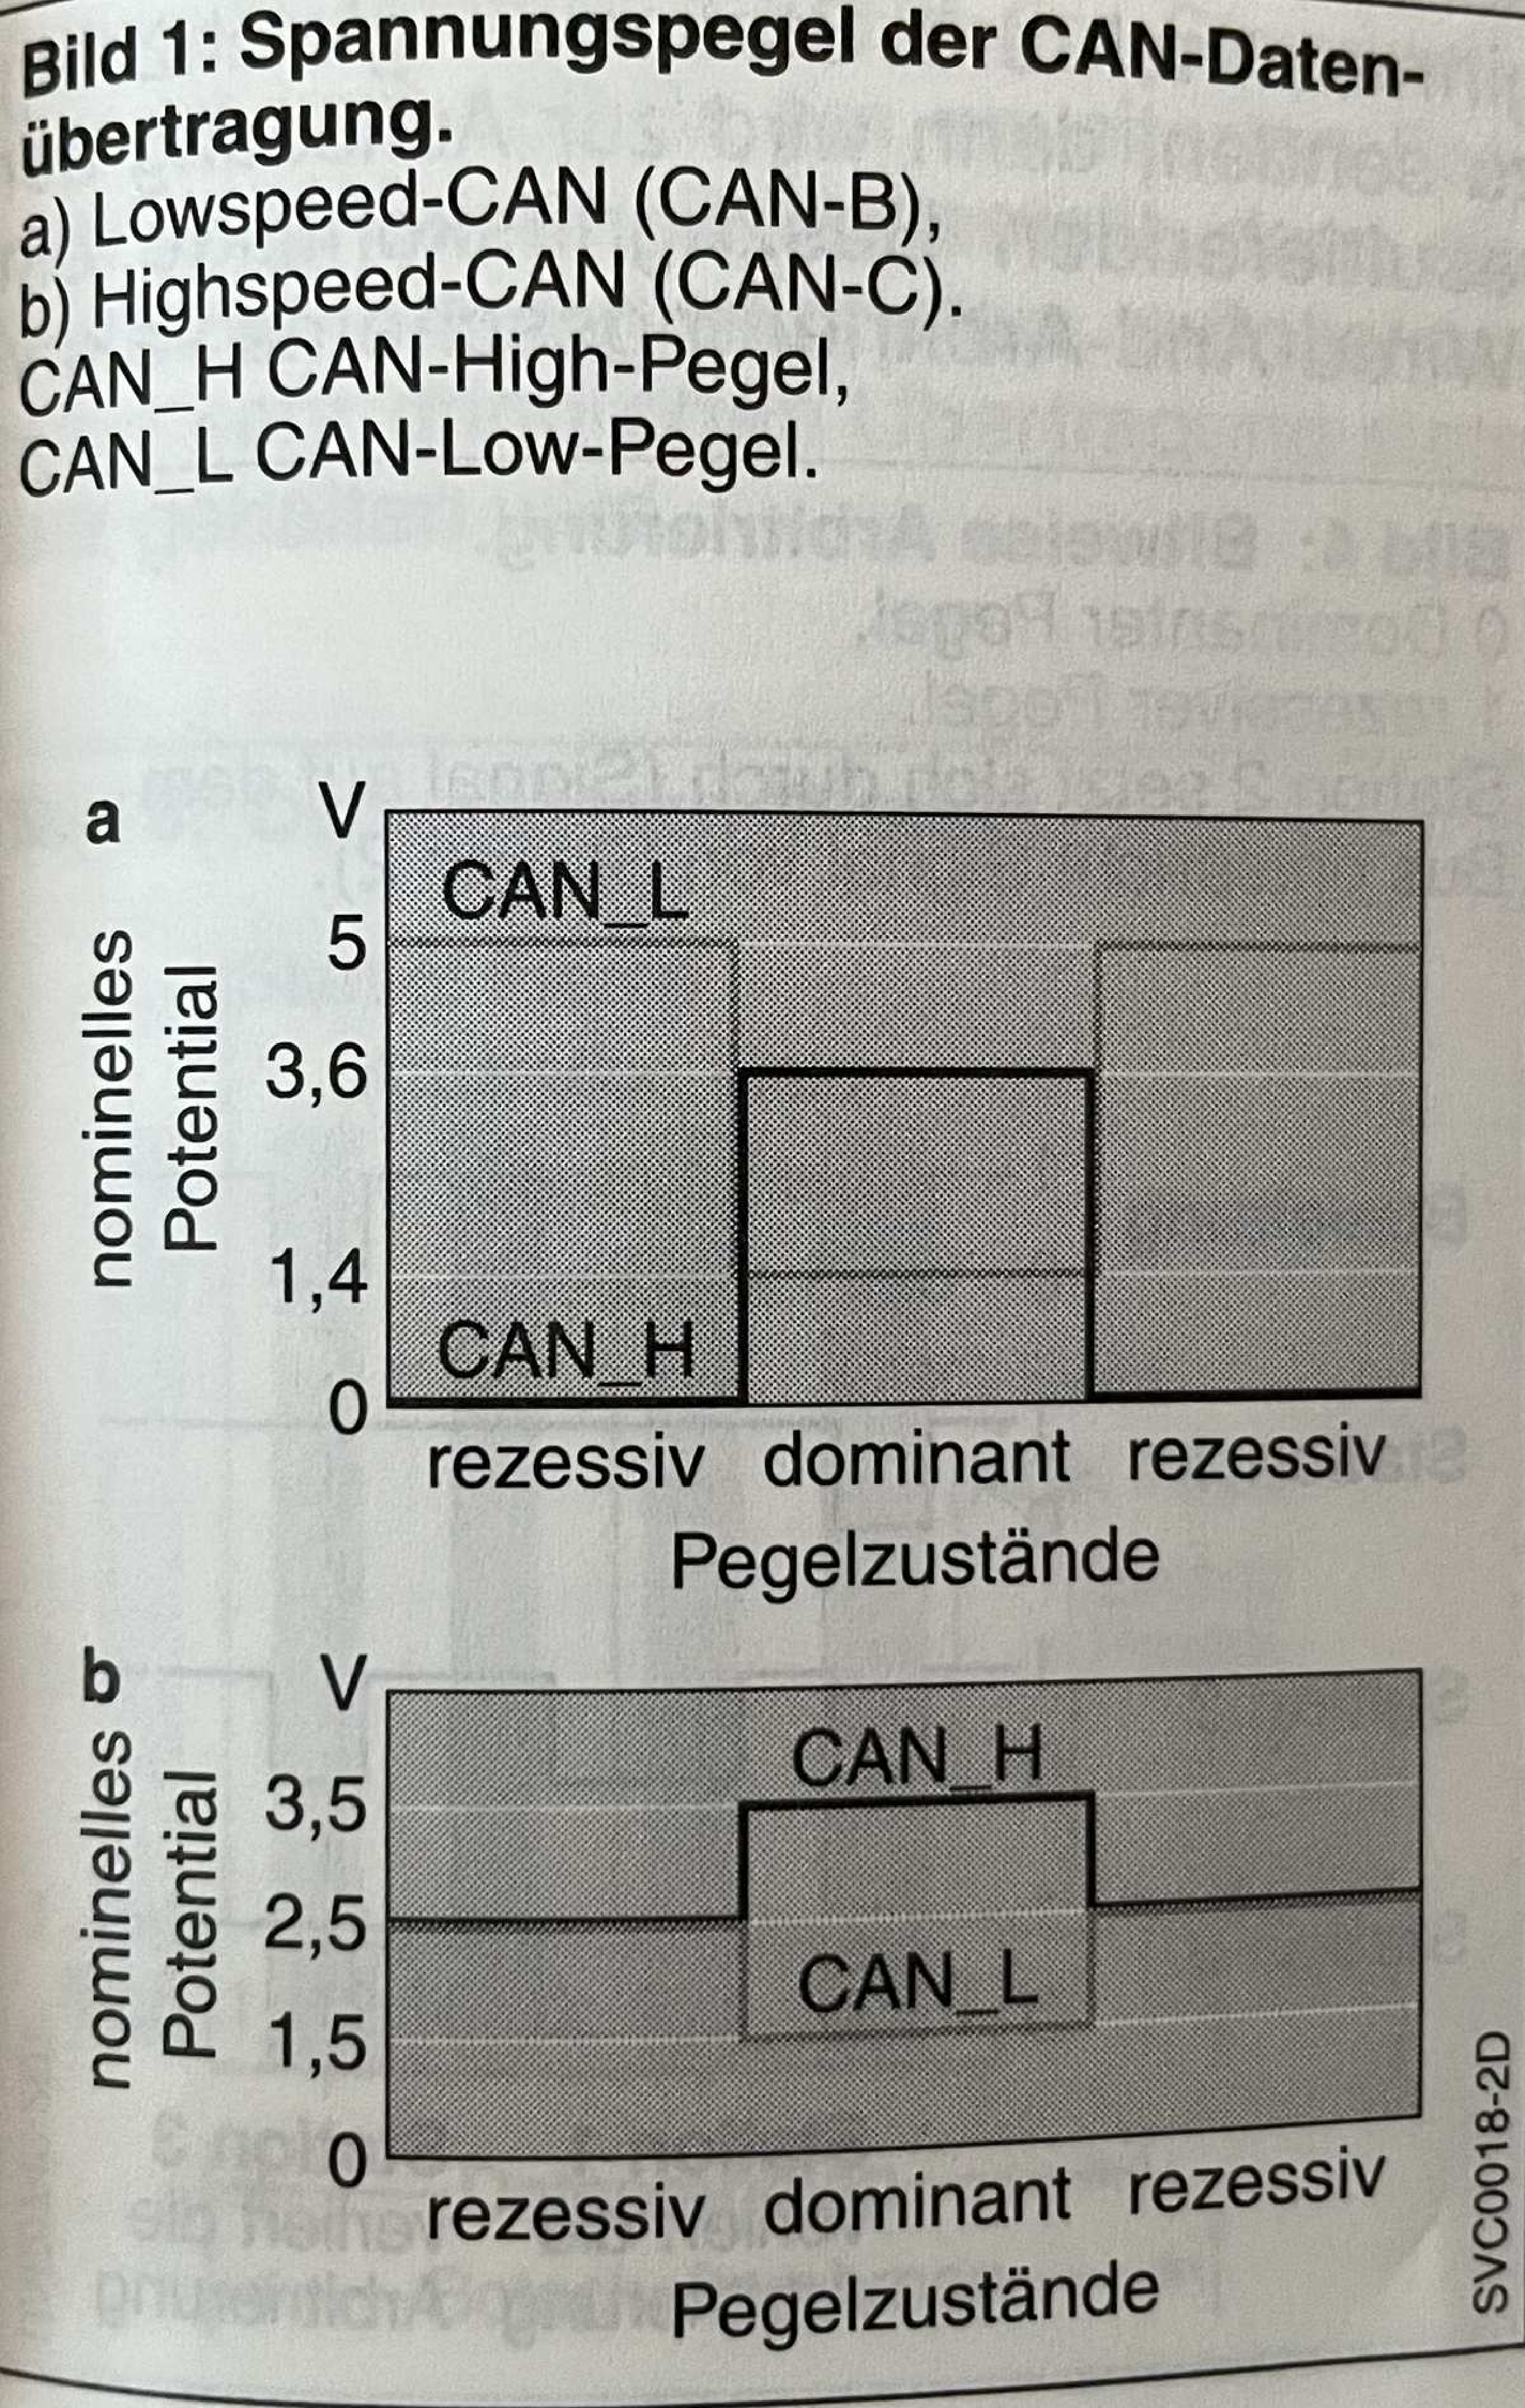
\includegraphics[width=0.4\textwidth]{images/CAN-Bus/CAN-Bus-11.pdf}
\caption{Spannungspegel, Quelle: Bosch}
%\label{fig:}%% anpassen
\end{figure}

\textbf{Steuern} >>dominant<< 0 überschreibt immer >>rezessiv<< 1 (tritt
zurück)

(dominant hat Vorrang, dann Datenübertragung)

\newpage

\section{Aufbau CAN-Nachricht -
Datenprotokoll}\label{aufbau-can-nachricht-datenprotokoll}

Das Datenprotokoll bestimmt den Aufbau der Datenbotschaft und ist
einheitlich festgelegt.

\begin{figure}[!ht]% hier: !ht
\centering
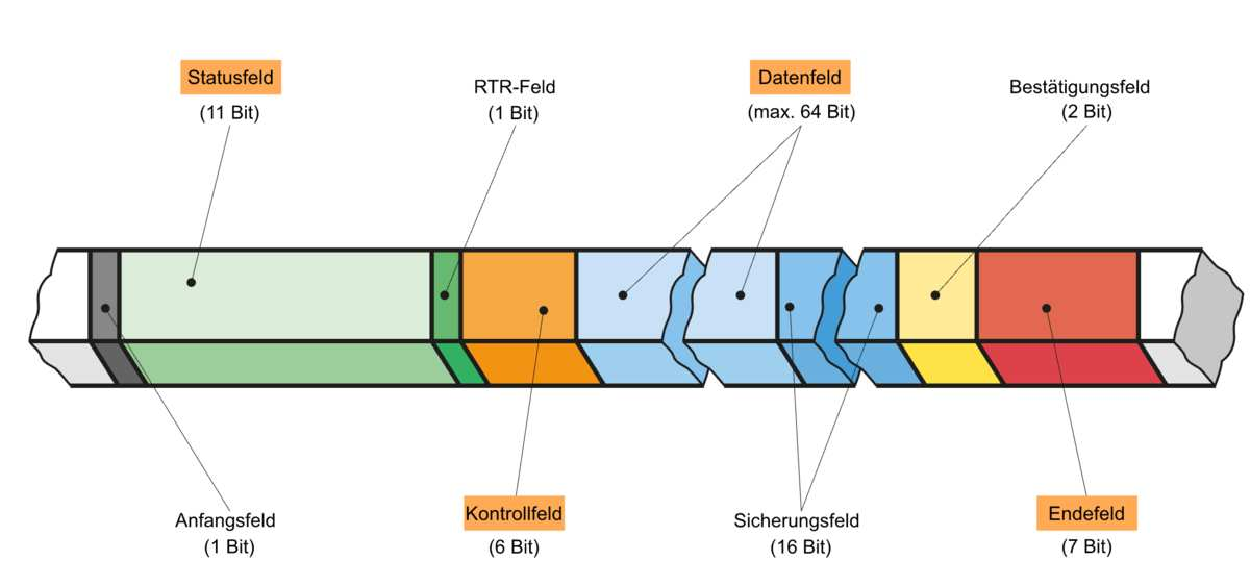
\includegraphics[width=0.6\textwidth]{images/CAN-Bus/CAN-Bus-1.pdf}
\caption{Aufbau CAN-Botschaft, Quelle: Europa-Verlag}
%\label{fig:}%% anpassen
\end{figure}

\begin{enumerate}
\item
  Anfangsfeld (1 Bit)

  \begin{itemize}
  \item
    Beginn der Botschaft
  \end{itemize}
\item
  Statusfeld (11 Bit) Identifier

  \begin{itemize}
  \item
    Botschaftsname (Beispiel: Motordaten)
  \item
    Je niedriger die Zahl, desto wichtiger die Nachricht.
  \item
    höchste Priorität vs.~geringste Priorität
  \item
    wichtige Daten vs.~weniger wichtige Daten
  \end{itemize}
\item
  RTR (1 Bit) Remote Transmission Request Feld

  \begin{itemize}
  \item
    \textbf{0} Senden und \textbf{1} Gib mir Daten
  \end{itemize}
\item
  Kontrollfeld (6 Bit)

  \begin{itemize}
  \item
    Enthält Prüfsumme
  \end{itemize}
\item
  Datenfeld (max. 64 Bit)

  \begin{itemize}
  \item
    Motordrehzahl, Motormoment, Motortemperatur usw.
  \end{itemize}
\item
  Sicherungsfeld (16 Bit)
\item
  Bestätigungsfeld (2 Bit)
\item
  Ende (7 Bit)

  \begin{itemize}
  \item
    der Nachricht, Bus wieder frei
  \end{itemize}
\end{enumerate}

\newpage

\section{Binärzahlen umwandeln}\label{binaerzahlen-umwandeln}

\textbf{Was ist die kleinste Informationseinheit bei der
Datenübertragung?} Bit

\textbf{Wie viele Informationen können mit einem Bit übertragen werden?}
Es können zwei Informationen übertragen werden.

\lstset{language=Python}% C, TeX, Bash, Python 
\begin{lstlisting}[
	%caption={}, label={code:}%% anpassen
]
// Beispiel: 8 bit = 256 (Anzahl der Informationen)
1 Bit = 0,1 2^1 = 2
2 Bit = 00,01,10,11 2^2 = 4
3 Bit = 000,001,011,111,110,100,101,010 2^3 = 8
1 Byte = 8 bit
2^8 = 256
2^16 = 65536 
\end{lstlisting}

\textbf{Zweier Potenzen}

$2^0 = 1 \\ 2^1 = 2 \\2^2 = 4 \\2^3 = 8 \\2^4 = 16 \\2^5 = 32 \\2^6 = 64 \\2^7 = 128 \\2^8 = 256$

\textbf{Binär in Dezimal}

\lstset{language=Python}% C, TeX, Bash, Python 
\begin{lstlisting}[
	%caption={}, label={code:}%% anpassen
]
 1 0 1 1 1 // Binärzahl (5-stellig)
16 8 4 2 1 // 2-Potenz
16 0 4 2 1 // Addieren
__________
Dezimal: 23
\end{lstlisting}

\textbf{Dezimal in Binär}

\lstset{language=Python}% C, TeX, Bash, Python 
\begin{lstlisting}[
	%caption={}, label={code:}%% anpassen
]
Dezimal: 99
Test 99 < 128        // also 7-stellige Binärzahl
64 32 16  8  4  2  1 // 2-Potenz
64+32                // Addieren
96             +2 +1 
 1  1  0  0  0  1  1 // Binärzahl 
\end{lstlisting}

\newpage

\section{Fehler am CAN-Bus}\label{fehler-am-can-bus}

Messung am OBD-Stecker direkt machen.

\textbf{Messpunkte} CAN-High (PIN 6) und CAN-Low (PIN 14)

\textbf{Gutbild} (CAN-Low-Signal \& CAN-High-Signal sind
spiegelverkehrt)

\begin{figure}[!ht]% hier: !ht
\centering
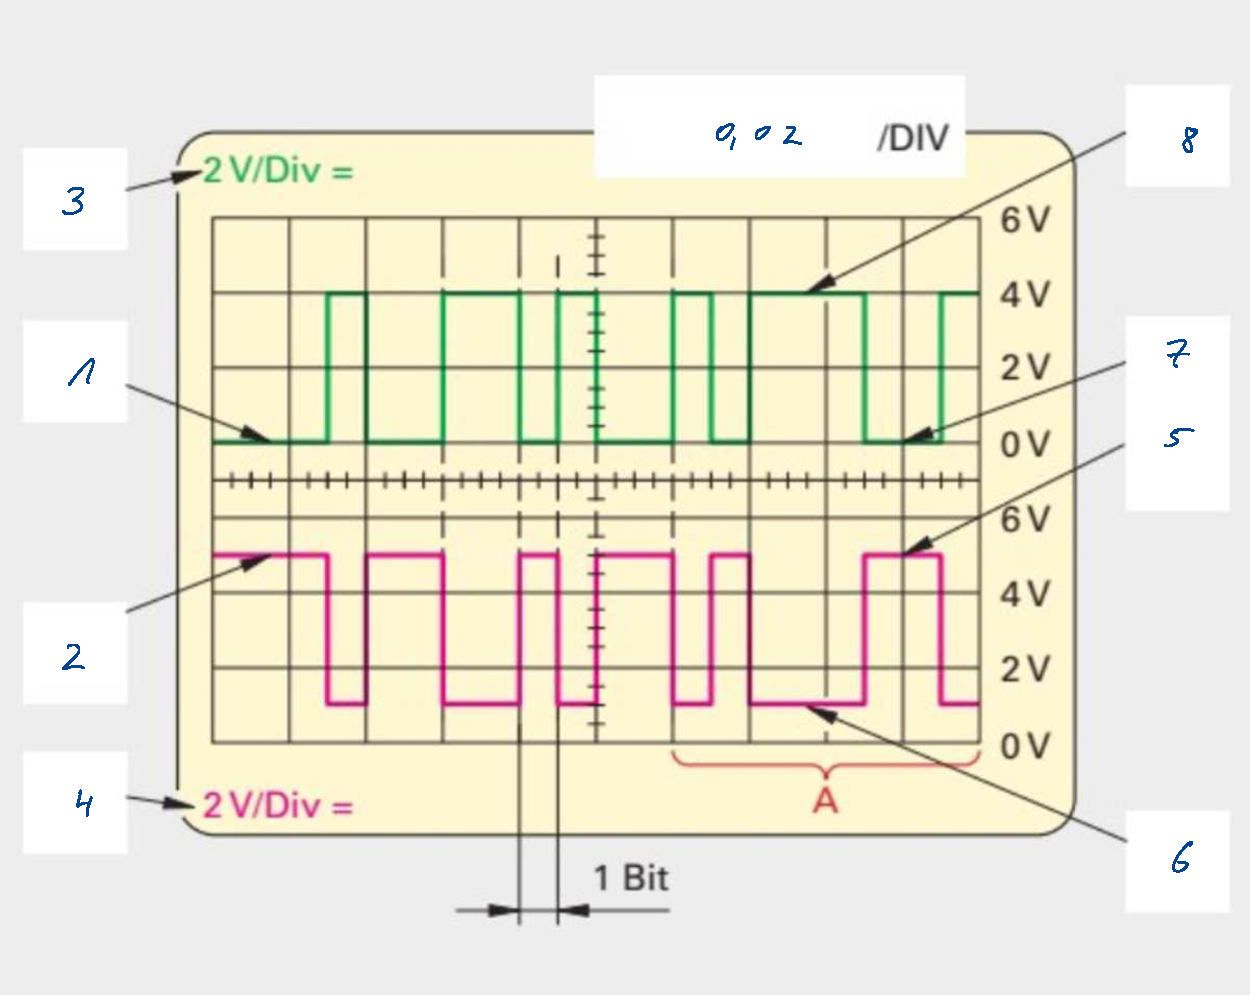
\includegraphics[width=0.4\textwidth]{images/CAN-Bus/CAN-Bus-4.pdf}
\caption{CAN-Bus, Quelle: Europa-Verlag}
%\label{fig:}%% anpassen
\end{figure}

\begin{enumerate}
\item
  Signal CAN - High
\item
  Signal CAN - Low
\item
  Einstellung Spannung/Division Kanal1
\item
  Einstellung Spannung/Division Kanal2
\item
  CAN-Low, rezessiver Pegel, Bit 1
\item
  CAN-Low, dominanter Pegel, Bit 0
\item
  CAN-High, rezessiver Pegel, Bit 1
\item
  CAN-High, dominanter Pegel, Bit 0
\end{enumerate}

\begin{figure}[!ht]% hier: !ht
\centering
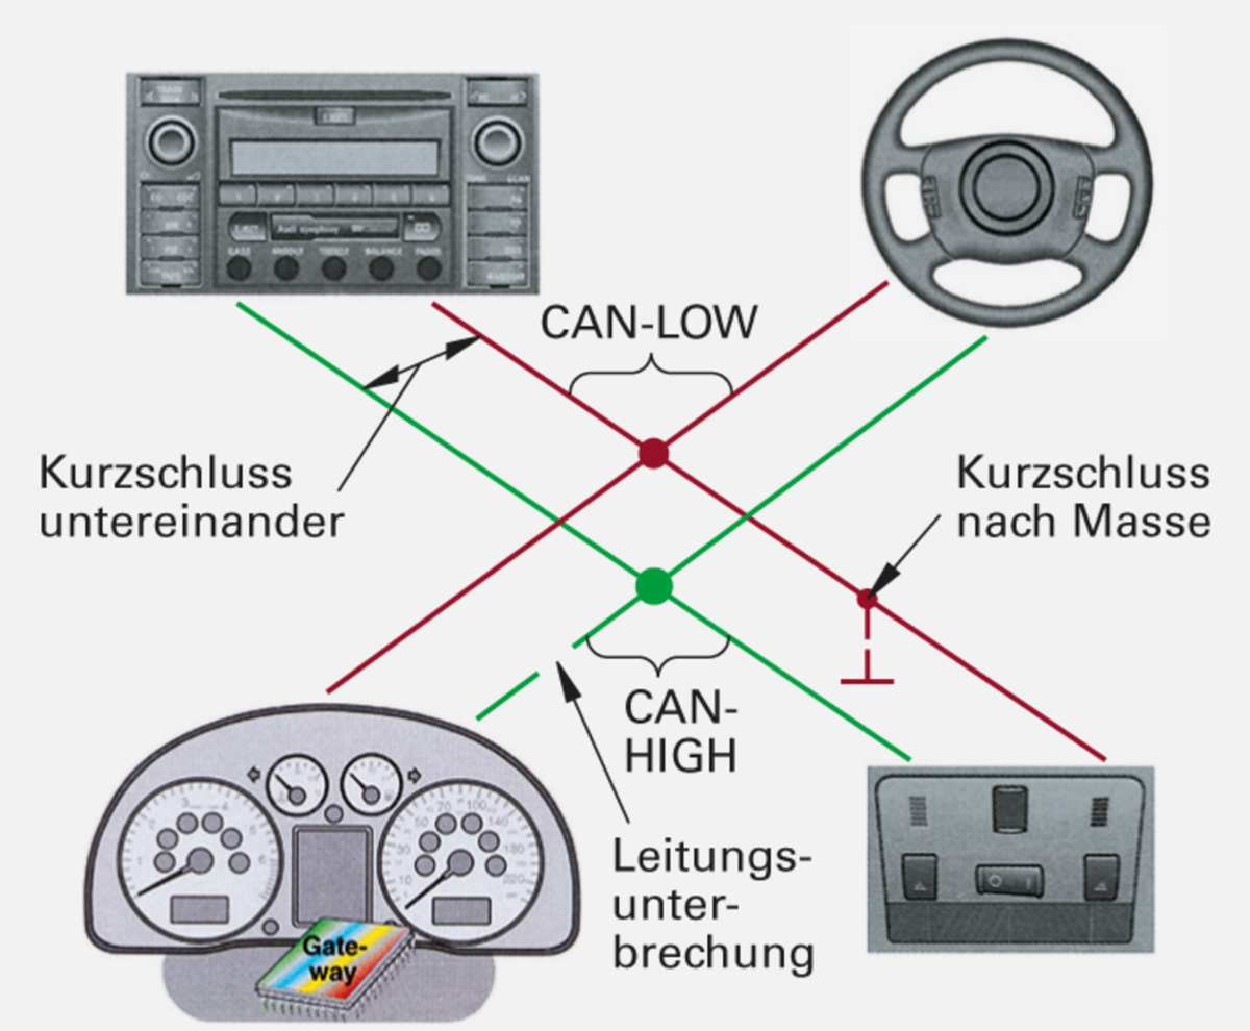
\includegraphics[width=0.4\textwidth]{images/CAN-Bus/CAN-Bus-10.pdf}
\caption{Fehlermöglichkeiten CAN-Bus, Quelle: Europa-Verlag}
%\label{fig:}%% anpassen
\end{figure}

\begin{figure}[!ht]% hier: !ht
\centering
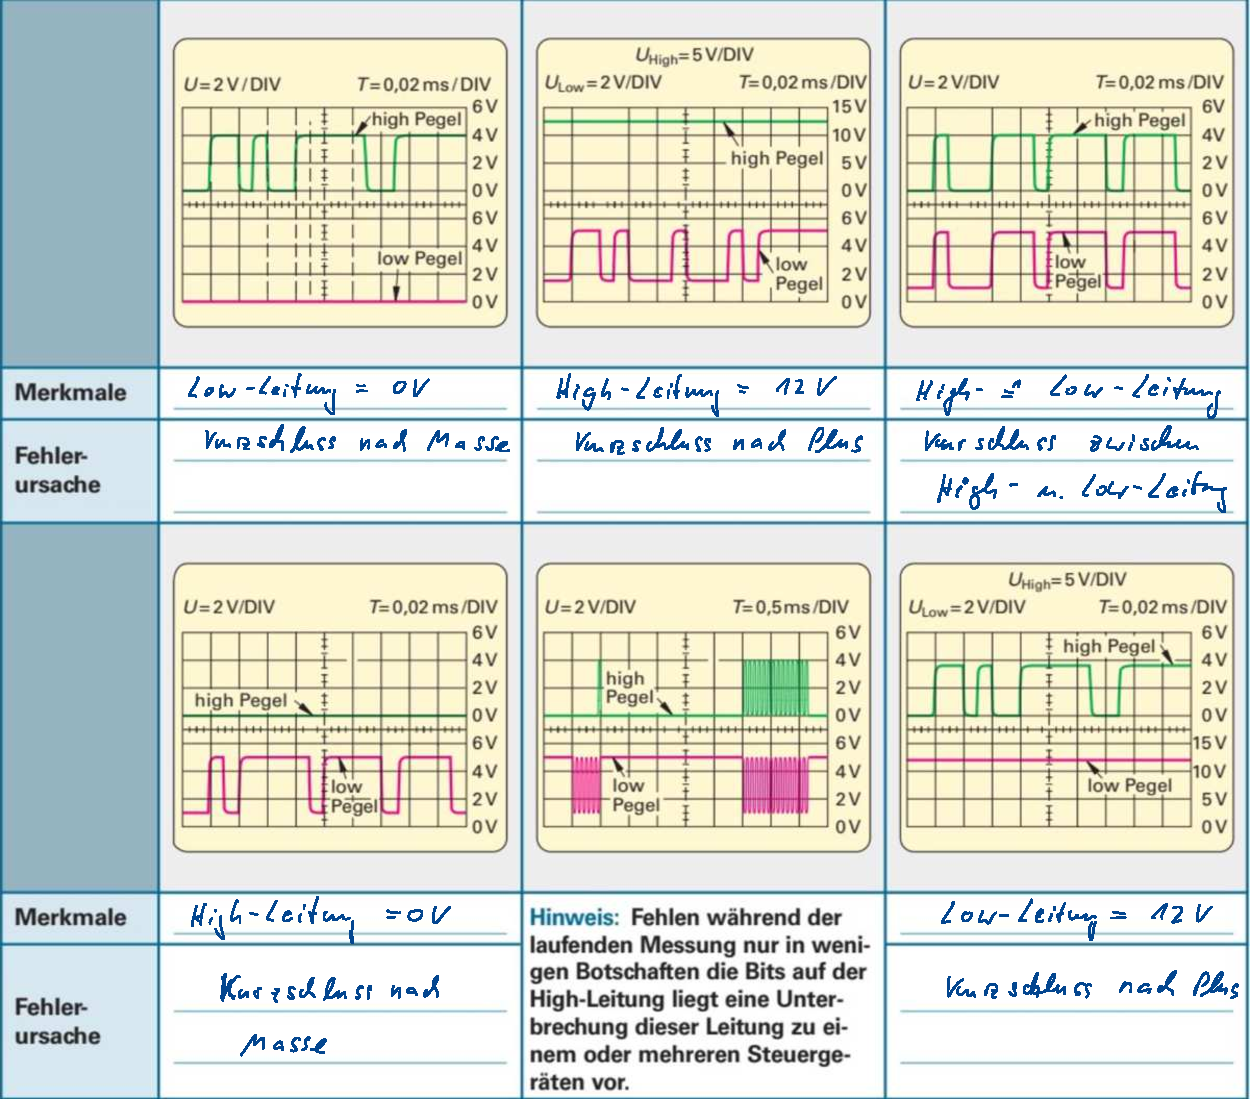
\includegraphics[width=0.8\textwidth]{images/CAN-Bus/CAN-Bus-5.pdf}
\caption{Fehler CAN-Bus, Quelle: Europa-Verlag}
%\label{fig:}%% anpassen
\end{figure}

\newpage

\subsection{Keine Kommunikation zum SG
möglich}\label{keine-kommunikation-zum-sg-moeglich}

\begin{enumerate}
\item
  CAN-High überprüfen

  \begin{itemize}
  \item
    \textbf{Messpunkt:} Oszi an (Pin6 \& Masse)
  \end{itemize}
\item
  CAN-Low überprüfen

  \begin{itemize}
  \item
    \textbf{Messpunkt:} Oszi an (Pin14 \& Masse)
  \end{itemize}
\end{enumerate}

\textbf{kein Spannungsverlauf?}

\begin{itemize}
\item
  Beide Leitungen durchmessen
\item
  CAN-High (SG gegen Masse)
\item
  CAN-Low (SG gegen Masse)
\end{itemize}
